\documentclass[preprint,12pt,a4paper]{elsarticle}
\usepackage{lmodern}
\usepackage{amssymb}
\usepackage{booktabs}
\usepackage{tabularx}
\usepackage{graphicx}
\usepackage{tikz}
\usepackage{float}
\usepackage{array}
\usepackage[table]{xcolor}
\usepackage{placeins}
\usepackage{caption}
\usepackage{hyperref}

\usetikzlibrary{arrows.meta,positioning,fit,shapes.geometric}
\setlength{\parindent}{0pt}
\setlength{\emergencystretch}{2em}
\newcolumntype{L}[1]{>{\raggedright\arraybackslash}p{#1}}
\newcolumntype{Y}{>{\raggedright\arraybackslash}X}
\newcommand{\tablerowsep}{\addlinespace[2pt]}
\newcommand{\figurepanellabel}[1]{\par{\footnotesize #1}}
\raggedbottom
\setcounter{topnumber}{4}
\setcounter{bottomnumber}{3}
\setcounter{totalnumber}{6}
\renewcommand{\topfraction}{0.95}
\renewcommand{\bottomfraction}{0.85}
\renewcommand{\textfraction}{0.05}
\renewcommand{\floatpagefraction}{0.95}
\setlength{\textfloatsep}{12pt plus 2pt minus 2pt}
\setlength{\floatsep}{10pt plus 2pt minus 2pt}
\setlength{\intextsep}{10pt plus 2pt minus 2pt}
\captionsetup{font=small,skip=6pt}
\makeatletter
\setlength{\@fptop}{0pt}
\setlength{\@fpsep}{10pt}
\setlength{\@fpbot}{0pt plus 1fil}
\setlength{\@dblfptop}{0pt}
\setlength{\@dblfpsep}{10pt}
\setlength{\@dblfpbot}{0pt plus 1fil}
\makeatother
\journal{SoftwareX}

% Generated by the release pipeline. The fallbacks keep draft builds readable,
% while check_softwarex_release.py rejects them for publication.
\IfFileExists{generated/release_metadata.tex}{\newcommand{\ReleaseVersion}{v1.0.2}
\newcommand{\ReleaseDOI}{10.5281/zenodo.21846125}
\newcommand{\ReleaseDate}{2026-08-08}
}{
  \newcommand{\ReleaseVersion}{v1.0.0 release candidate}
  \newcommand{\ReleaseDOI}{release gate pending}
  \newcommand{\ReleaseDate}{release gate pending}
}

\begin{document}
\begin{frontmatter}

\title{Medora: A Consent-Aware Bilingual Platform for Healthcare Management and Consultation with Assistive AI}

\author{Sarwad Hasan Siddiqui}
\author{Adiba Tahsin}
\author{Kazi Saeed Alam\corref{cor1}}
\ead{saeed.alam@cse.kuet.ac.bd}
\cortext[cor1]{Corresponding author.}
\author{Sk. Imran Hossain}
\address{Department of Computer Science and Engineering, Khulna University of Engineering \& Technology, Khulna 9203, Bangladesh}

\begin{abstract}
Medora is an English/Bengali, consent-aware platform combining patient-held records,
appointment coordination, and 21 assistive-AI endpoints in an installable progressive web
application. Patients describe concerns by text or voice to discover doctors; clinicians
receive structured intake, source-linked histories, speech-to-notes, and reviewable drafts.
Chorui guides both roles through registered workflows. External processing requires
purpose-specific revocable consent, redaction, and pseudonymization. These controls reduce
exposure without establishing anonymity. Transactional booking
coordinates concurrent requests and post-commit notifications. The historical Bangladesh
medicine reference contains 7,389 drugs and 67,001 brands; a revision rebuild adds row-level
source attribution and change records. A prescription prototype integrates region detection,
OCR, parsing, and catalog matching. Reproducibility artifacts document privacy, navigation,
summary, and booking behaviour. Medora supports software research and human-reviewed
workflows; clinical effectiveness is outside this evaluation.

\end{abstract}

\begin{keyword}
digital health \sep assistive AI \sep consent-gated processing \sep
medicine reference data \sep deterministic intent routing \sep bilingual software
\end{keyword}
\end{frontmatter}

\section*{Code metadata}
The code metadata required for reproducibility is summarized in [\hyperref[codeMetadata]{Table~\ref*{codeMetadata}}].

\begin{table}[!htbp]
\caption{Code metadata. The archived release date is \ReleaseDate.}
\label{codeMetadata}
\small
\begin{tabular}{@{}L{0.05\textwidth}L{0.35\textwidth}L{0.53\textwidth}@{}}
\toprule
\textbf{Nr.} & \textbf{Description} & \textbf{Value} \\
\midrule
C1 & Current code version & \ReleaseVersion \\
\tablerowsep
C2 & Permanent link to code/repository used for this code version & \url{https://github.com/CSE-3200-System-Project/Medora/tree/\ReleaseVersion}; archive \ReleaseDOI \\
\tablerowsep
C3 & Permanent link to Reproducible Capsule & Code Ocean capsule; permanent URL to be added after the reproducibility pass. \\
\tablerowsep
C4 & Legal Code License & Project source: MIT; combined detector distribution: AGPL-3.0 with corresponding source and preserved notices \\
\tablerowsep
C5 & Code versioning system used & Git \\
\tablerowsep
C6 & Software code languages, tools, and services used & Python, TypeScript, SQL; FastAPI, Next.js, PostgreSQL; hosted text models (Groq, Gemini, Cerebras) with a deterministic mock; optional faster-whisper, Vapi, PaddleOCR, and Azure Document Intelligence \\
\tablerowsep
C7 & Compilation requirements, operating environments \& dependencies & Python 3.11, Node.js 20, PostgreSQL 16, or checksummed containers; reference deployment on Vercel and Azure Container Apps \\
\tablerowsep
C8 & If available Link to developer documentation/manual & \url{https://github.com/CSE-3200-System-Project/Medora/tree/main/docs} \\
\tablerowsep
C9 & Support email for questions & saeed.alam@cse.kuet.ac.bd \\
\bottomrule
\end{tabular}

\end{table}


\section{Motivation and significance}

Medora connects bilingual records, discovery, booking, summaries, voice and medicine
lookup under shared authorization and audit controls for health-informatics researchers
and educators.


Bangladesh eHealth studies identify opportunities to strengthen implementation and
record adoption~\cite{ahmed2014,khan2012}. Medora connects patient-held information to
bilingual search, appointments, and record views under user control.

First, a shared Bangladesh medicine reference supports lookup, prescribing, histories
and OCR matching. RxNorm does not cover Bangladesh~\cite{rxnorm}. The revision builder
consolidates four of five inventoried sources into generic, brand and typo-tolerant
search tables, preserving source rows and transformations.


Second, patients describe conditions by text or voice to obtain specialty-oriented
doctor candidates. Source-linked summaries organize supplied records; Chorui reaches
registered workflows through chat, speech, or Vapi. Clinicians receive intake, consultation,
dictation, record-review, and prescribing support.

Third, consent precedes external calls, a fixed registry bounds navigation, and
backend-attached references link summaries to supplied records. Deterministic controls
(Table~\ref{tab:components}) keep access, routes, and clinical writeback outside model authority.


OpenMRS, Bahmni, and GNU Health provide broad institutional record, hospital, laboratory,
and FHIR capabilities~\cite{openmrs,bahmni,gnuhealth}. Medora complements them with a
compact mobile client connecting patient-held records and transactional booking to
bilingual assistive AI (Table~\ref{tab:related-work}).

Clinical-summary studies assess correctness and completeness beyond fluency; clinician--AI
trials show task- and workflow-dependent effects~\cite{shing2021,tracsum,zhang2024clinicalsummary,goh2025gpt4assistance}.
Bangla-HealthNER documents informal, code-mixed health text~\cite{khan2023banglahealthner}.
Re-identification and prompt-injection studies motivate explicit processing boundaries
~\cite{campion2025diri,yang2025adversarial}; symptom-checker studies motivate careful urgency
handling~\cite{wallace2022}. Medora links summaries to supplied records, presents specialty
candidates rather than diagnoses, and retains manual browsing.

\begin{table}[!htbp]
\caption{Scope comparison from project documentation. Cells summarize documented emphasis and do not imply that unlisted capabilities are absent.}
\label{tab:related-work}
\scriptsize
\setlength{\tabcolsep}{3pt}
\begin{tabularx}{\textwidth}{@{}L{0.19\textwidth}YYYY@{}}
\toprule
\textbf{Criterion} & \textbf{OpenMRS}\cite{openmrs} & \textbf{Bahmni}\cite{bahmni} & \textbf{GNU Health}\cite{gnuhealth} & \textbf{Medora} \\
\midrule
Deployment & Modular server platform & Multi-service hospital distribution & Integrated hospital system & Three-service research stack \\
\tablerowsep
Patient mobile workflow & Deployment-specific web clients & Hospital-oriented web workflows & Web and desktop clients & English/Bengali patient PWA \\
\tablerowsep
Booking and live slots & Scheduling modules; deployment-specific updates & Appointment workflows & Appointment management & Transactional booking; post-commit updates \\
\tablerowsep
Assistive AI & Outside this comparison scope & Outside this comparison scope & Outside this comparison scope & 21 endpoints; text/voice assistance; source-linked drafts \\
\tablerowsep
Medicine reference & Deployment-supplied dictionaries & Deployment-supplied dictionaries & Deployment-supplied dictionaries & Shared Bangladesh index; attributed revision builder \\
\tablerowsep
Consent and audit & Privilege and audit modules & OpenMRS roles and audit tools & Role and audit tools & Purpose-, provider-, and scope-specific grants \\
\tablerowsep
Bengali localization & Localization framework & Localization support & Localization framework & Bundled English and Bengali catalogs \\
\tablerowsep
Interoperability & REST/FHIR ecosystem & OpenMRS interoperability ecosystem & FHIR and health standards & JSON/REST contracts; FHIR mapping is future work \\
\tablerowsep
Release status & Open source; mature deployments & Open source; hospital deployments & Open source; international deployments & Research release; licences in C4 \\
\bottomrule
\end{tabularx}

\end{table}

\section{Software description}

\subsection{Software architecture}

Medora comprises a Next.js web client, a FastAPI core API, a separate FastAPI OCR service,
and PostgreSQL (Fig.~\ref{fig:trust}). Authentication identifies the actor; backend checks
of role, ownership, care relationship, appointment state, and consent authorize each
operation. Frontend visibility is only a usability aid.

The reference deployment at \url{https://medorahealth.vercel.app/} uses Vercel for the
frontend and Azure Container Apps for the backend. Archived containers provide the
reproducible release environment.

Authorization is checked at both API and database boundaries. The release restricts
anonymous direct-data access, enables row-level security, and exposes a trigger-maintained
change feed. Access-denial tests cover requests that bypass frontend controls.

\begin{figure}[!htbp]
\centering\resizebox{\textwidth}{!}{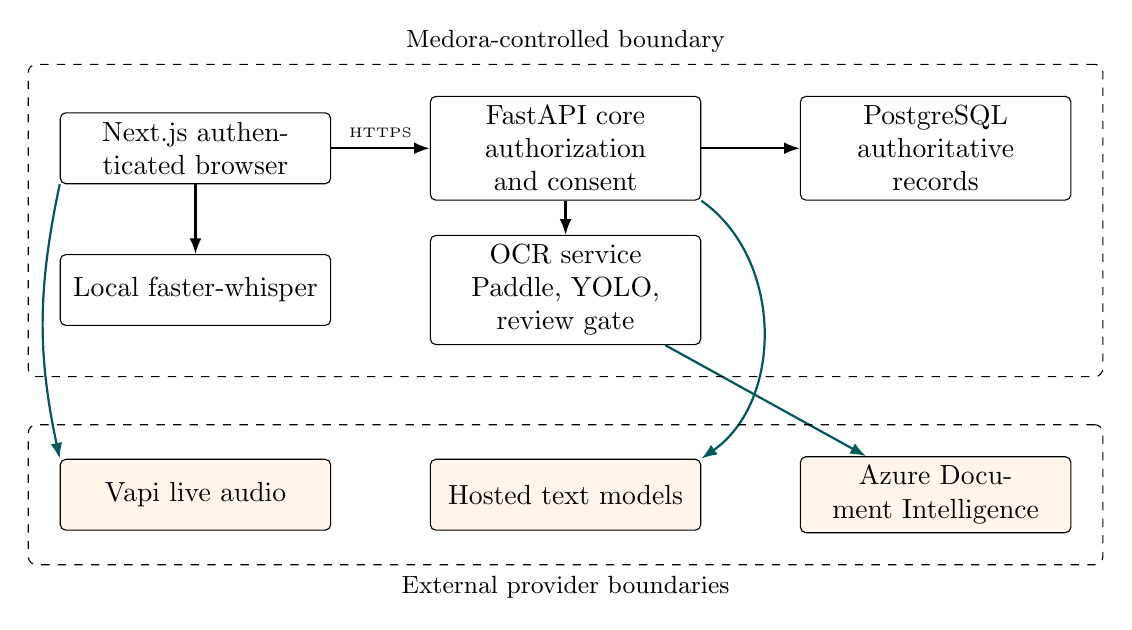
\begin{tikzpicture}[
  box/.style={draw, rounded corners=2pt, align=center, minimum height=9mm, text width=32mm, fill=white},
  boundary/.style={draw, dashed, rounded corners=3pt, inner sep=4mm},
  flow/.style={-{Latex[length=2mm]}, thick},
  consent/.style={-{Latex[length=2mm]}, thick, teal!70!black},
  external/.style={draw, rounded corners=2pt, align=center, minimum height=9mm, text width=32mm, fill=orange!8},
  grant/.style={font=\scriptsize, fill=white, inner sep=1.5pt, text=teal!70!black}
]
\node[box] (browser) at (0,0) {Next.js authenticated browser};
\node[box] (backend) at (4.7,0) {FastAPI core\\authorization and consent};
\node[box] (db) at (9.4,0) {PostgreSQL\\authoritative records};
\node[box] (whisper) at (0,-1.8) {Local faster-whisper};
\node[box] (ocr) at (4.7,-1.8) {OCR service\\Paddle, YOLO, review gate};

\node[external] (vapi) at (0,-4.4) {Vapi live audio};
\node[external] (llm) at (4.7,-4.4) {Hosted text models};
\node[external] (azure) at (9.4,-4.4) {Azure Document Intelligence};

\draw[flow] (browser) -- node[above, font=\tiny]{HTTPS} (backend);
\draw[flow] (backend) -- (db);
\draw[flow] (backend) -- (ocr);
\draw[flow] (browser) -- (whisper);
\draw[consent] (browser.south west) to[bend right=12] (vapi.north west);
\draw[consent] (backend.south east) to[out=-35,in=35] (llm.north east);
\draw[consent] (ocr) -- (azure);

\node[boundary, fit=(browser)(backend)(db)(ocr)(whisper)] (medora-boundary) {};
\node[font=\small, fill=white, inner sep=1pt, anchor=south]
  at ([yshift=1mm]medora-boundary.north) {Medora-controlled boundary};
\node[boundary, fit=(vapi)(llm)(azure)] (provider-boundary) {};
\node[font=\small, fill=white, inner sep=1pt, anchor=north]
  at ([yshift=-1mm]provider-boundary.south) {External provider boundaries};
\end{tikzpicture}
}
\caption{Deployment and trust boundaries. Local speech recognition and local OCR remain
inside the Medora boundary. Hosted text models, Vapi live audio, and Azure OCR are separate
recipients with separate grants.}
\label{fig:trust}
\end{figure}

Consent-aware processing is deny-by-default (Fig.~\ref{fig:consent}). Grants record subject,
recipient, purpose, scopes, policy version, validity, revocation, and audit metadata. Invalid
grants receive an explanation and, where available, a local alternative. Revocation blocks
future processing, not past disclosure; local mode never silently escalates to cloud processing. Provider-
and purpose-specific grants distinguish hosted text, Vapi audio, and Azure OCR processing.

Medora exposes JSON/REST contracts and PDF output. Human-readable sharing controls map
to machine-readable grants; missing external-processing consent returns HTTP 403.
gICS and the Greifswald trusted-third-party dispatcher demonstrate consent exchange and
modular pseudonymization services~\cite{gics2022,ttp2024}. Medora's local guards provide an
adapter boundary, not those services. Future FHIR Consent/IHE PCF exchange requires profiles,
terminology bindings and transactions~\cite{fhirconsent,ihepcf,consent2025}; no standards
conformance is claimed.

For EU use, health data remain special-category personal data after pseudonymization.
Deployment-specific review must establish lawful basis, an Article 9 condition,
processor/transfer/retention arrangements, data-subject workflows, and any required DPIA
~\cite{gdpr}. MDR classification depends on intended purpose, with separate clinical-investigation
obligations; German AMG provisions govern medicinal-product trials~\cite{mdr,amg}.
These requirements need assessment before such deployment; Medora makes no regulatory
compliance claim.

\begin{figure}[!htbp]
\centering\resizebox{\textwidth}{!}{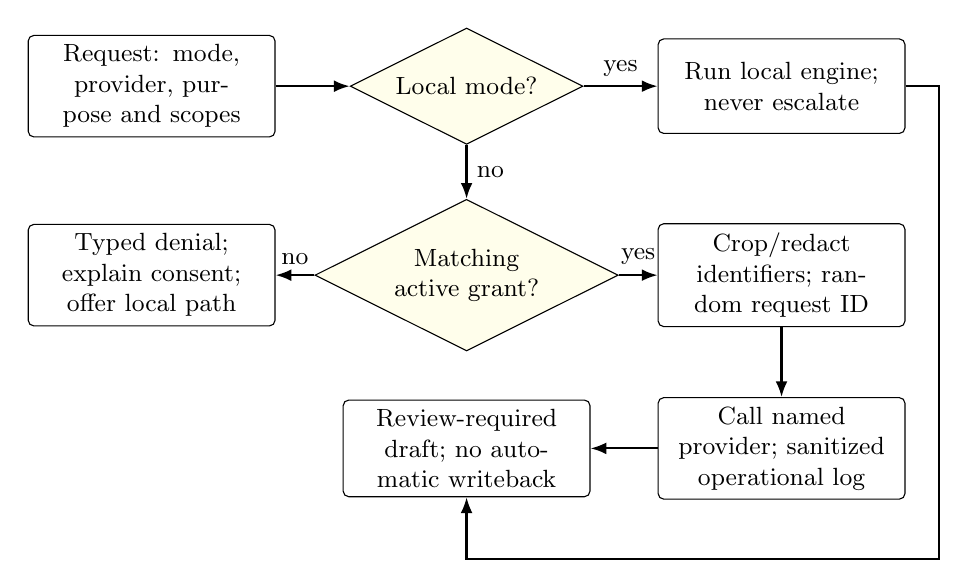
\begin{tikzpicture}[
  font=\small,
  flowbox/.style={draw, rounded corners=2pt, align=center, minimum height=12mm, text width=29mm, fill=white},
  decision/.style={draw, diamond, aspect=2.0, align=center, text width=22mm, inner sep=1.5pt, fill=yellow!8},
  flow/.style={-{Latex[length=2mm]}, thick}
]
\node[flowbox] (request) at (0,0) {Request: mode, provider, purpose and scopes};
\node[decision] (local) at (4,0) {Local mode?};
\node[flowbox] (localrun) at (8,0) {Run local engine; never escalate};
\node[decision] (grant) at (4,-2.4) {Matching active grant?};
\node[flowbox] (deny) at (0,-2.4) {Typed denial; explain consent; offer local path};
\node[flowbox] (redact) at (8,-2.4) {Crop/redact identifiers; random request ID};
\node[flowbox] (provider) at (8,-4.6) {Call named provider; sanitized operational log};
\node[flowbox] (draft) at (4,-4.6) {Review-required draft; no automatic writeback};
\draw[flow] (request) -- (local);
\draw[flow] (local) -- node[above]{yes} (localrun);
\draw[flow] (local) -- node[right]{no} (grant);
\draw[flow] (grant) -- node[above]{yes} (redact);
\draw[flow] (grant) -- node[above]{no} (deny);
\draw[flow] (redact) -- (provider);
\draw[flow] (provider) -- (draft);
\draw[flow] (localrun.east) -- (10,0) -- (10,-6) -- (4,-6) -- (draft.south);
\end{tikzpicture}
}
\caption{Consent-aware processing. Purpose and provider are checked before any external
call, and outputs return as review-ready drafts.}
\label{fig:consent}
\end{figure}

\subsection{Software functionalities}

\textbf{Bangladesh medicine reference.} Three shared tables support lookup
(Table~\ref{tab:corpus}): \texttt{drugs} stores generic--strength--form identities,
\texttt{brands} maps commercial names, and \texttt{medicine\_search\_index} supports
trigram-based typo tolerance. Search, prescribing, histories, and OCR matching use this
identity layer.

The revision rebuild yields 46,614 rows, 6,153 drug identities, 52,767 search terms, and
72,969 source-row links. It records file hashes, row numbers, field contributors, and exact
transformations. Conservative whitespace normalization and duplicate reconciliation
preserve ingredient and strength text; conflicting identities and unparsed records are
quarantined. Indication prose is excluded. Independent replay reproduces all output hashes.
This prospective rebuild documents its own lineage, not the historical CSV's missing links.
Historical runtime counts remain distinct. Multi-source publication follows source-permission
documentation; dosage recommendations and interaction checking remain separate extensions.

\begin{table}[!htbp]
\caption{Historical medicine reference as loaded. Canonical keys collapse brand duplicates. The separately attributed revision rebuild has 46,614 rows and 6,153 drug identities; it has not replaced this runtime corpus.}
\label{tab:corpus}
\centering
\small

\renewcommand{\arraystretch}{1.15}
\setlength{\tabcolsep}{6pt}

\begin{tabular}{@{}lr@{}}

\toprule
\textbf{Artifact} & \textbf{Count} \\
\midrule

Consolidated source rows
& 71{,}795 \\[2pt]

Canonical drugs (generic $\times$ strength $\times$ form)
& 7{,}389 \\[2pt]

Brand entries
& 67{,}001 \\[2pt]

Search-index terms
& 74{,}390 \\[2pt]

Distinct generic names
& 5{,}242 \\[2pt]

Distinct brand names
& 52{,}117 \\

\bottomrule

\end{tabular}

\end{table}

\textbf{Assistive-AI layer.} Twenty-one endpoints cover doctor discovery, summaries, intake,
consultation, references, speech-to-notes, safety checks, and live voice
(Table~\ref{tab:ai-surface}). One provider-agnostic orchestrator supports Groq, Gemini,
Cerebras, and a deterministic mock. It sanitizes input, assigns a random correlation ID,
schema-validates responses, and records operational metadata, allowing providers to change
without rewriting workflows. Typed responses enforce application contracts; malformed output is rejected.

Before orchestration, consent filters permitted categories and marks partial records; a
bilingual redactor removes known identifiers; and pseudonymization replaces patient IDs.
Raw clinical content is excluded from default logs. Clinician access also requires a care
relationship and appears in the patient's audit view. Tests exercise these shared privacy and authorization stages.
The threat model covers unauthorized access and external disclosure: TLS, managed storage,
secret custody, provider retention and audit privileges have deployment-specific assumptions.
The archived security assessment distinguishes access logging from tamper-proof auditing.

\begin{table}[!htbp]
\caption{AI and machine-learning components. Thirteen of nineteen use deterministic logic;
the remaining six coordinate or perform language, speech, and image-model inference.}
\label{tab:components}
\scriptsize
\setlength{\tabcolsep}{4pt}
\begin{tabularx}{\textwidth}{@{}>{\hsize=.80\hsize\raggedright\arraybackslash}X>{\hsize=.66\hsize\raggedright\arraybackslash}X>{\hsize=1.94\hsize\raggedright\arraybackslash}X>{\hsize=.60\hsize\raggedright\arraybackslash}X@{}}
\toprule
\textbf{Component} & \textbf{Kind} & \textbf{Role} & \textbf{Model} \\
\midrule
AI orchestrator & Interface & Provider-agnostic call path: sanitize, dispatch, schema-validate, log latency & Yes \\
\tablerowsep
Consent guard & Deterministic & Resolves permitted data categories; filters payload; emits restriction notice & No \\
\tablerowsep
Bilingual redactor & Deterministic & Pattern removal of contact, identity, address, and date spans in Bengali and English & No \\
\tablerowsep
Patient pseudonymiser & Deterministic & Stable opaque reference replacing raw identifiers & No \\
\tablerowsep
Processing-consent service & Deterministic & Purpose-, provider-, and scope-scoped external grants with revocation & No \\
\tablerowsep
Chorui intent normalizer & Deterministic & Utterance to canonical intent, bilingual & No \\
\tablerowsep
Chorui route registry & Deterministic & Immutable role-scoped intent-to-route table; admin routes absent & No \\
\tablerowsep
Chorui navigation engine & Deterministic & Role-aware resolution, missing-parameter clarification, fallbacks & No \\
\tablerowsep
Specialty matcher & Deterministic & Exact, synonym, fuzzy, and similarity matching of specialty terms & No \\
\tablerowsep
Medical knowledge base & Deterministic & Symptom-to-specialty relations and universal fallback chains & No \\
\tablerowsep
Emergency red-flag rules & Deterministic & Keyword screen that pre-empts model output with emergency guidance & No \\
\tablerowsep
Speech recognition (faster-whisper) & Local model & Bilingual transcription of clinician dictation & Yes, local \\
\tablerowsep
Live-voice bridge (Vapi) & External & Tool-calling surface resolving through the same registry and guards & Yes, external \\
\tablerowsep
Dosage matcher & Deterministic & Dosage, frequency, duration, and quantity grammar & No \\
\tablerowsep
Medicine fuzzy matcher & Deterministic & Trigram and edit-distance matching against the reference index & No \\
\tablerowsep
Region detector (YOLO) & Local model & Prescription region localisation & Yes, local \\
\tablerowsep
Local OCR (PaddleOCR) & Local model & On-premise text recognition & Yes, local \\
\tablerowsep
Cloud OCR (Azure) & External & Optional recognition backend under a separate grant & Yes, external \\
\tablerowsep
Report and prescription parsers & Deterministic & Structured extraction of test results and medication rows & No \\
\bottomrule
\end{tabularx}

\end{table}

Figure~\ref{fig:chorui} summarizes the assistant's deterministic request path.

\begin{figure}[!htbp]
\centering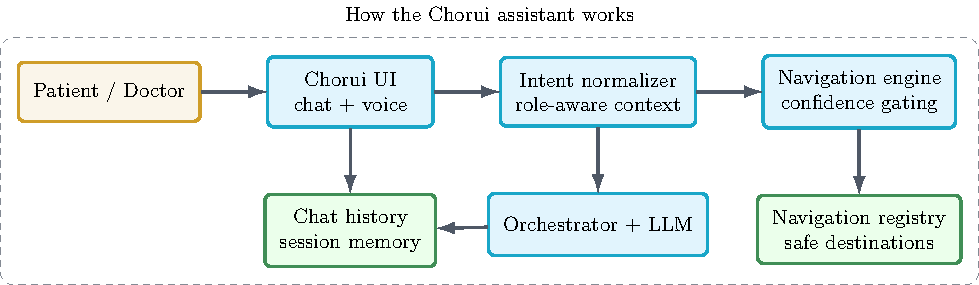
\includegraphics[width=\textwidth]{figures-src/chorui_architecture.pdf}
\caption{Chorui request path. Text or voice requests receive conversational phrasing while
deterministic intent normalization and registry resolution select role-appropriate app
destinations.}
\label{fig:chorui}
\end{figure}

\begin{table}[!htbp]
\caption{The assistive-AI surface. Shared processing applies consent checks, redaction,
pseudonymization, and schema validation. Navigation and summaries have task-specific
fixtures across three groups; the other six are documented capabilities. Paths, schemas,
authorization rules, and examples are retained in the API specification.}
\label{tab:ai-surface}
\centering
\scriptsize

\renewcommand{\arraystretch}{1.18}
\setlength{\tabcolsep}{4pt}

\begin{tabularx}{\textwidth}{
@{}
>{\raggedright\arraybackslash}p{0.23\textwidth}
>{\centering\arraybackslash}p{0.04\textwidth}
>{\raggedright\arraybackslash}X
>{\raggedright\arraybackslash}p{0.15\textwidth}
@{}
}

\toprule
\textbf{Endpoint group} &
\textbf{No.} &
\textbf{User-facing contribution} &
\textbf{Task evidence} \\
\midrule

Assistant chat and conversations
& 4
& Bilingual help, conversation history, and guided navigation
& Navigation fixtures \\[2pt]

Specialty and doctor search
& 1
& Condition-to-specialty doctor candidates
& Navigation fixtures \\[2pt]

Record summarisation
& 3
& Source-linked patient and prescription histories
& Summary fixtures \\[2pt]

Intake structuring
& 2
& Confirmable structured intake drafts
& Capability \\[2pt]

Consultation assistance
& 6
& Reviewable notes, queries, summaries, and prescription drafts
& Capability \\[2pt]

Clinical reference query
& 1
& Structured reference text with confidence and cautions
& Capability \\[2pt]

Speech to notes
& 1
& Bilingual dictation to editable clinical forms
& Capability \\[2pt]

Safety check
& 1
& Advisory flags inside the clinician workflow
& Capability \\[2pt]

Live voice tool calls
& 2
& Vapi conversation with role-aware tools
& Capability \\[3pt]

\midrule

\textbf{Total}
& \textbf{21}
&
& \textbf{3 fixture groups} \\

\bottomrule

\end{tabularx}

\end{table}

\textbf{Chorui assistant.} Bengali/English text and voice requests resolve through a fixed
registry: 23 canonical intents in 24 entries, comprising 11 patient, 11
clinician, and 2 shared. Entries bind routes, parameters and fallbacks. Missing details
trigger clarification; unregistered administrative routes remain unreachable.
Chat and Vapi use the same auditable resolution path.

\textbf{Summaries and speech.} Medora organizes patient, clinician, and prescription
histories into role-specific, read-only summaries. Backend-attached references keep every
item traceable to supplied records and allow return to the underlying entry. Empty source
sets produce a not-found result, and summaries never write back automatically. The current
summary payload omits dates, so these summaries are not evaluated as chronological histories. Local
faster-whisper supports bilingual dictation~\cite{whisper}; Vapi adds live conversation and
the same Chorui and doctor-search tools under a separate live-audio grant.

\textbf{Human-centered workflow.} Summaries remain reviewable, prescription suggestions
pre-fill fields a prescriber edits and signs, and specialty search retains direct browsing.
OCR produces row-by-row drafts marked \texttt{authoritative\_writeback=false}; patients may
acknowledge receipt or report discrepancies without implying clinical endorsement. These
review points keep decisions and changes with users.

\textbf{Installable bilingual client.} The PWA supports English and Bengali, standalone
display, maskable icons, and home-screen installation. Browser tests cover both locales.
Only public/versioned resources are cached; health writes stay online, and logout clears
caches, IndexedDB, and sensitive storage.

\textbf{Reliable appointments.} Idempotency keys, row locks, availability checks and
uniqueness constraints protect booking. Appointment, audit, replay result and outbox event
commit together; clients recover PostgreSQL state after reconnection. Reminders use in-app
notifications, email and optional web push.

\subsection{Evaluation and reproducibility}

Evaluation covers privacy, navigation, summary references and booking concurrency.
Mock and recorded-provider results are separated.

The hand-authored bilingual privacy suite covers identifiers
(Table~\ref{tab:privacy-span-results}), spelling and spacing variants, obfuscation,
over-redaction, consent, and prompt injection. It exercises the production path without
supplying known identifiers to the redactor.
The frozen v1.0.2 report records 71 true positives, 4 false positives, and 23 false negatives
over 94 expected spans (94.7\% precision, 75.5\% recall, and 3.2\% false redaction).
These frozen-fixture results are not independently held-out evidence or measurements of
later changes. Residual disclosure includes prose names, month-name dates, and obfuscated
contacts; consent and pseudonymization remain necessary at the provider boundary.

Navigation fixtures separate recorded-provider and mock paths, scoring against the request
path's classifier. The deterministic emergency screen has
TP=7, FN=0, FP=5, and TN=18; Table~\ref{tab:navigation-emergency-results} reports
sensitivity, specificity, positive predictive value, and negative predictive value with
two-sided 95\% Wilson intervals. Uncertainty accompanies candidates; manual browsing stays available. The screen
also matches some negated, third-person, and historical mentions. These clinician-reviewed
fixtures are preliminary software checks, not clinical triage accuracy.
Mock summary fixtures check supplied-record references, not-found results for empty input,
and rejection of malformed output.

Consent, redaction, route allowlisting, and schemas are software invariants; no
LLM-only/deterministic-only/hybrid ablation or clinical-output comparison was performed.

Completed component experiments extend this evidence (Table~\ref{tab:privacy-extension}).
Rules, optional MuRIL (threshold 0.30), and their union are compared on the development
suite and a separate 36-case synthetic probe, including three Bengali cases. Probe recall
is 75.0\%, 97.2\%, and 100.0\%, respectively. Development results also show the union's
higher false-redaction rate; they do not establish naturalistic bilingual generalization.
The 24-case consent experiment varies records and redaction (Table~\ref{tab:consent-scope}):
L omits records, K adds reference context, R shares three categories, H shares all six,
and U computes unredacted exposure offline. Its contract utility measures source accounting.

Booking contention comprised 30 fresh-slot trials per level (2, 10, 50 requests), plus one
excluded warm-up. Each required one persisted winner, expected conflicts, idempotent replay,
mismatched-key rejection, and outbox processing. Table~\ref{tab:booking-results} reports n
and nearest-rank p50/p95/p99 for transaction and outbox latency. Environment, raw observations,
and 95\% trial-cluster bootstrap intervals are archived. In-process ASGI timings are not
deployed-capacity estimates.

\IfFileExists{generated/safety_results.tex}{\begin{table}[!h]
\centering\small
\resizebox{\linewidth}{!}{%
\begin{tabular}{@{}lrll@{}}
\toprule
Suite & Cases & Reported measurement & Scope \\
\midrule
Bilingual privacy & 134 & recall 75.5\% (95\% CI 66.0--83.1\%); TP=71, FP=4, FN=23 & synthetic \\
Symptom navigation & 30 & emergency sensitivity 7/7 (95\% CI 64.6--100.0\%); FP=5 & complete \\
Source-grounded summaries & 12 & 12/12 fixture assertions & deterministic mock \\
\bottomrule
\end{tabular}%
}
\caption{Fixture measurements. Privacy counts are span-level; intervals are two-sided Wilson 95\% intervals on fixture denominators, not population or clinical-performance estimates. Fixture assertions and documented limitations are release-audit properties, not evidence that all cases were correct. Detection rates are in Table~\ref{tab:privacy-span-results}.}
\label{tab:safety-results}
\end{table}
\begin{table}[!h]
\centering\small
\begin{tabular}{@{}lrrl@{}}
\toprule
Measure & n & N & Estimate (95\% Wilson CI) \\
\midrule
Sensitivity & 7 & 7 & 100.0\% (64.6--100.0\%) \\
Specificity & 18 & 23 & 78.3\% (58.1--90.3\%) \\
Positive predictive value & 7 & 12 & 58.3\% (32.0--80.7\%) \\
Negative predictive value & 18 & 18 & 100.0\% (82.4--100.0\%) \\
\bottomrule
\end{tabular}
\caption{Deterministic emergency screen on 30 clinician-reviewed fixtures: TP=7, FN=0, FP=5, TN=18. Wilson intervals describe fixtures only, not clinical triage performance.}
\label{tab:navigation-emergency-results}
\end{table}
\begin{table}[!h]
\centering\small
\begin{tabular}{@{}lrrrr@{}}
\toprule
Expected class & Cases & Recorded & Mock & Documented \\
\midrule
emergency & 7 & 7 & 7 & 0 \\
manual\_browse & 2 & 0 & 0 & 2 \\
specialty\_candidates & 16 & 10 & 6 & 5 \\
uncertain & 5 & 2 & 2 & 0 \\
\bottomrule
\end{tabular}
\caption{Provider-dependent specialty outcomes are separated from the deterministic emergency screen. Recorded and Mock are fixture paths and do not represent a live-provider comparison.}
\label{tab:navigation-agreement-results}
\end{table}
\begin{table*}[!ht]
\centering\scriptsize
\begin{tabular}{@{}lrrrrr@{}}
\toprule
Identifier group & Cases & Precision & Recall & False redaction & Documented limitations \\
\midrule
account\_id & 7 & 100.0\% & 71.4\% & 0.0\% & 3 \\
address & 7 & 100.0\% & 71.4\% & 0.0\% & 2 \\
benign & 21 & -- & -- & 14.3\% & 3 \\
clinician & 4 & 100.0\% & 20.0\% & 0.0\% & 3 \\
consent & 10 & -- & -- & -- & 0 \\
date & 6 & 100.0\% & 50.0\% & 0.0\% & 3 \\
email & 9 & 100.0\% & 55.6\% & 0.0\% & 4 \\
injection & 10 & 100.0\% & 100.0\% & 0.0\% & 0 \\
limitation & 10 & -- & -- & 0.0\% & 10 \\
mixed\_script & 4 & 100.0\% & 100.0\% & 0.0\% & 0 \\
name\_labeled & 11 & 90.9\% & 90.9\% & 9.1\% & 3 \\
name\_unlabeled & 5 & -- & 0.0\% & 0.0\% & 5 \\
national\_id & 9 & 100.0\% & 100.0\% & 0.0\% & 5 \\
opaque\_id & 4 & 100.0\% & 100.0\% & 0.0\% & 0 \\
passport & 6 & 100.0\% & 66.7\% & 0.0\% & 2 \\
phone & 11 & 100.0\% & 100.0\% & 0.0\% & 0 \\
\midrule
All production-path cases & 134 & 94.7\% & 75.5\% & 3.2\% & 43 \\
\bottomrule
\end{tabular}
\caption{Span-level privacy metrics on the production call path, which supplies the redactor with no known identifiers. A dash means the group annotates no span for that denominator. The undetected identifier forms are named in the text.}
\label{tab:privacy-span-results}
\end{table*}
}{}
\IfFileExists{generated/booking_results.tex}{\begin{table}[!h]
\centering\small
\resizebox{\linewidth}{!}{%
\begin{tabular}{@{}rrrll@{}}
\toprule
Attempts & Passed trials & HTTP n & Transaction p50/p95/p99 (ms) & Outbox n; p50/p95/p99 (ms) \\
\midrule
2 & 30 / 30 & 60 & 24.6 / 26.8 / 31.4 & 30; 44.2 / 51.7 / 54.2 \\
10 & 30 / 30 & 300 & 246.1 / 380.5 / 396.2 & 30; 377.8 / 428.4 / 452.0 \\
50 & 30 / 30 & 1500 & 860.2 / 1028.8 / 1094.0 & 30; 897.0 / 1003.4 / 1035.0 \\
\bottomrule
\end{tabular}%
}
\caption{Each independent fresh-slot trial sends N simultaneous attempts; one warm-up trial per level is excluded. Pass requires one persisted winner, correct conflicts, idempotent replay, mismatch rejection, and processed outbox. Transaction and post-commit propagation latency are distinct; nearest-rank p50/p95/p99 are descriptive and topology-specific.}
\label{tab:booking-results}
\end{table}
}{}
\IfFileExists{generated/extended_results.tex}{\begin{table}[!htbp]
\caption{Archived privacy-component comparison. Development results reuse the 134-case tuning set; the separate probe has 36 synthetic cases, 36 identifier spans and 36 benign spans. Recall intervals are two-sided Wilson 95\% intervals. These populations are not pooled or treated as clinical evidence.}
\label{tab:privacy-extension}
\centering\small\setlength{\tabcolsep}{3pt}
\begin{tabular}{@{}llrrr@{}}\toprule
Population & System & \shortstack{Precision\\(\%)} & \shortstack{Recall (\%)\\95\% CI} & \shortstack{False redaction\\(\%)} \\
\midrule
Development & Rules & 96.9 & 100.0 (96.1--100.0\%) & 2.4 \\
\midrule
Development & MuRIL & 93.1 & 100.0 (96.1--100.0\%) & 5.6 \\
\midrule
Development & Union & 93.1 & 100.0 (96.1--100.0\%) & 5.6 \\
\midrule
Separate probe & Rules & 100.0 & 75.0 (58.9--86.2\%) & 0.0 \\
\midrule
Separate probe & MuRIL & 100.0 & 97.2 (85.8--99.5\%) & 0.0 \\
\midrule
Separate probe & Union & 100.0 & 100.0 (90.4--100.0\%) & 0.0 \\
\bottomrule\end{tabular}
\end{table}
\begin{table}[!htbp]
\caption{Archived consent-scope experiment on 24 synthetic summaries. Utility is a binary source-accounting contract, not clinical quality. Exposure counts surviving identifiers offline per 1,000 requests; U is an offline exposure counterfactual, not unredacted provider disclosure. Aggregate-only observations do not support paired or causal inference.}
\label{tab:consent-scope}
\centering\small\begin{tabular}{@{}lrr@{}}\toprule
Configuration & Contract utility (\%) & Exposure /1,000 requests \\
\midrule
L & 0.0 & 0.0 \\
\midrule
L+K & 0.0 & 0.0 \\
\midrule
L+K+R & 33.3 & 958.3 \\
\midrule
L+K+R+H & 12.5 & 1958.3 \\
\midrule
U & 8.3 & 6000.0 \\
\bottomrule\end{tabular}
\end{table}
}{}

The provider manifest records configurations, dates, retention and service assumptions.
Recorded-provider fixtures use archived outputs; other adapters are unevaluated. The capsule
checks archived statistics and reruns current safety and isolated booking, preserving historical tables.
Commands, checksums and raw outputs are archived.
%

\textbf{Experimental prescription OCR.} Region detection, local/cloud recognition, dosage
parsing, Bengali numeral normalization and catalog matching produce reviewable drafts
~\cite{du2020,prescriptionocr}. Cursive text and partial tokens required manual correction.
Every row requires verification before saving; no task-accuracy benchmark is reported.

The YOLO26s model card records the authors' Roboflow v2 attribution, corrected Colab
recipe, artifact checksums and inspected metadata. PT settings agree with the notebook,
and all 204 matched named ONNX tensors agree exactly after fusion. This verifies current
parameter correspondence. Historical dataset linkage, differing validation logs and
runtime-output differences are documented separately; the check does not measure held-out
accuracy or full prediction equivalence. Approved weight distribution includes AGPL-3.0
corresponding source, while prescription images remain private.

\section{Illustrative examples}

The patient dashboard shows record coverage, $100n/4$, where $n$ counts measurement
groups with finite stored readings in today's UTC window up to the snapshot. Groups
comprise steps, sleep, heart rate, and blood pressure (requiring both components).
An adjacent panel lists their presence; an expandable disclosure explains inputs and
human-readable timestamps. Unavailable responses are distinguished from zero.
Coverage describes stored-data presence, not health or measurement quality, and does not
recommend recording all four groups.

Figures~\ref{fig:ui-bilingual}--\ref{fig:ui-ai} show the demonstration interfaces;
their provenance is described in the ethics statement.

\begin{figure}[!htbp]
\centering
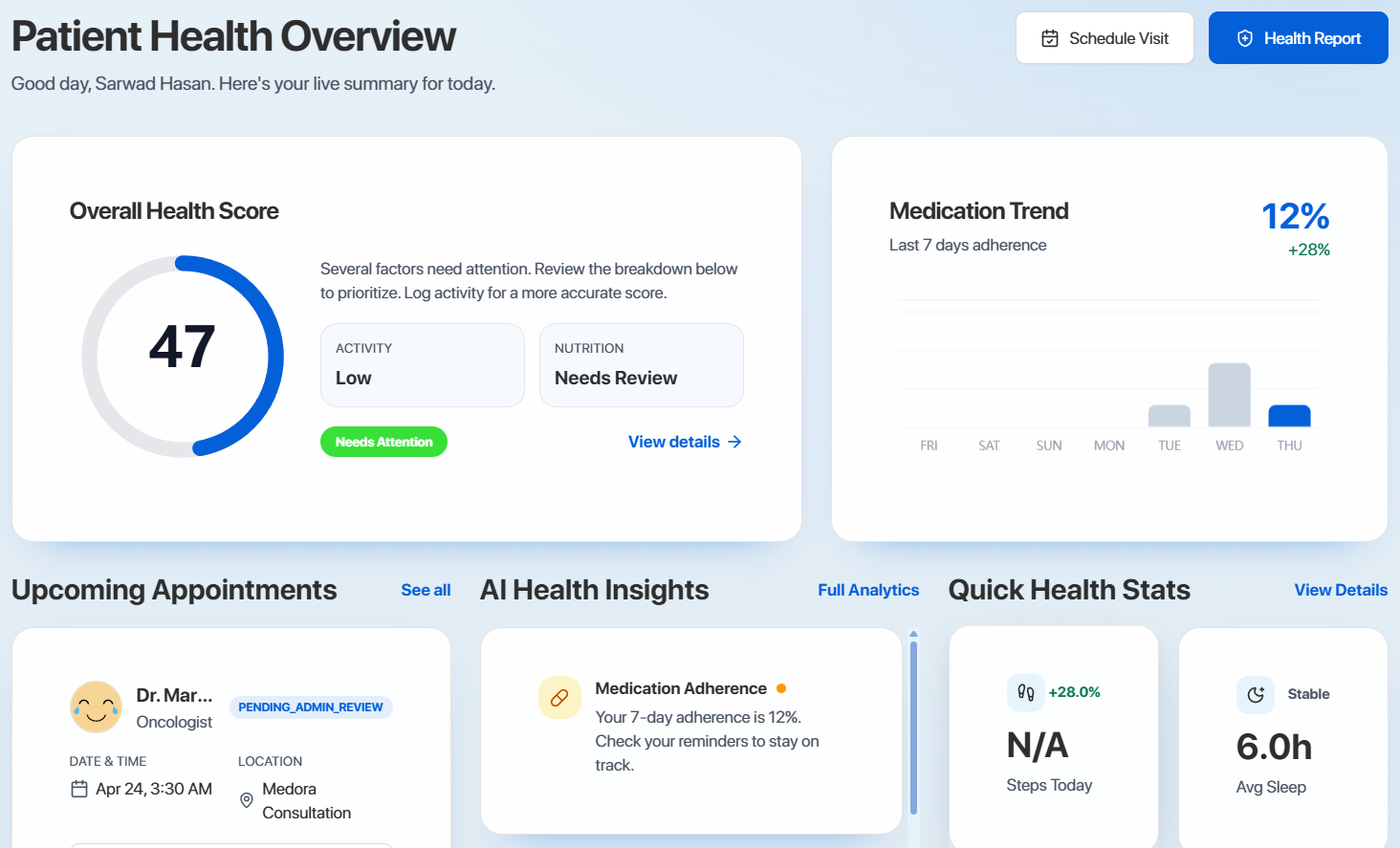
\includegraphics[width=\textwidth]{figures-ui/ui_dashboard_en.png}\\[3pt]
\figurepanellabel{(a) English}\vspace{6pt}
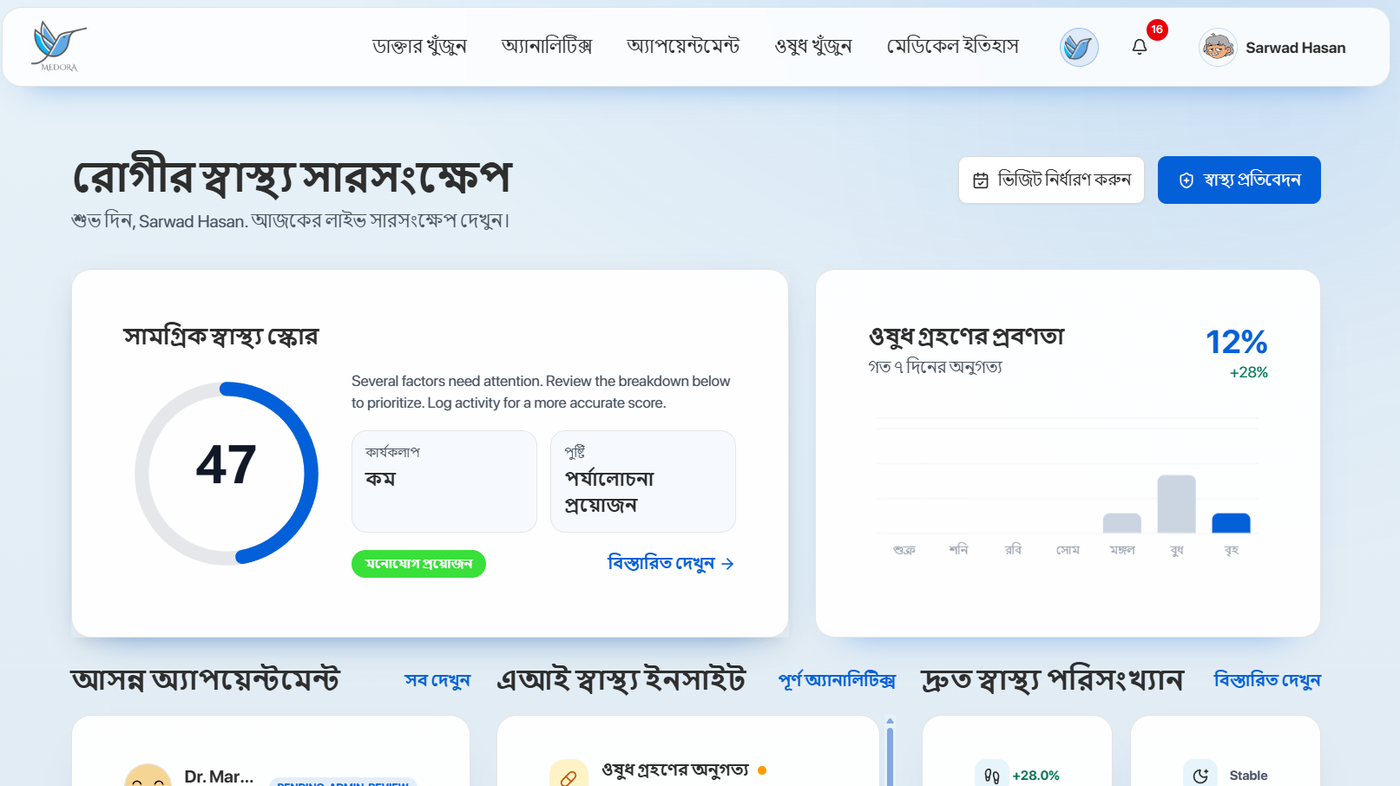
\includegraphics[width=\textwidth]{figures-ui/ui_dashboard_bn.png}\\[3pt]
\figurepanellabel{(b) Bengali}
\caption{Patient dashboard in (a) English and (b) Bengali, showing application navigation,
record coverage, and measurement-group status. Three of four groups contain records,
giving 75\% coverage. The expandable calculation explains inputs and the time window.
The percentage describes record presence, not clinical health.}

\label{fig:ui-bilingual}
\end{figure}

\begin{figure}[!htbp]
\centering
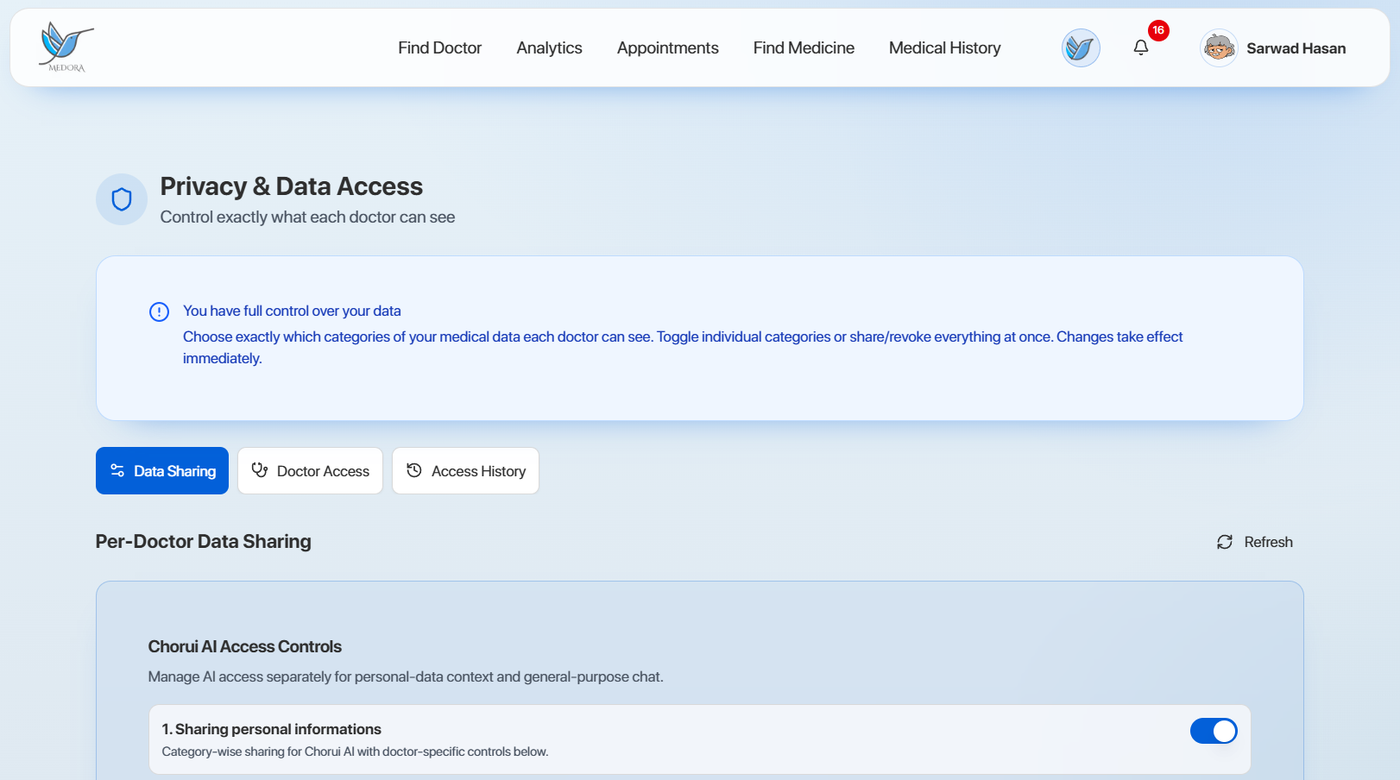
\includegraphics[width=0.80\textwidth]{figures-ui/ui_consent_sharing.png}\\[3pt]
\figurepanellabel{(a) Per-recipient, per-category sharing}\vspace{6pt}
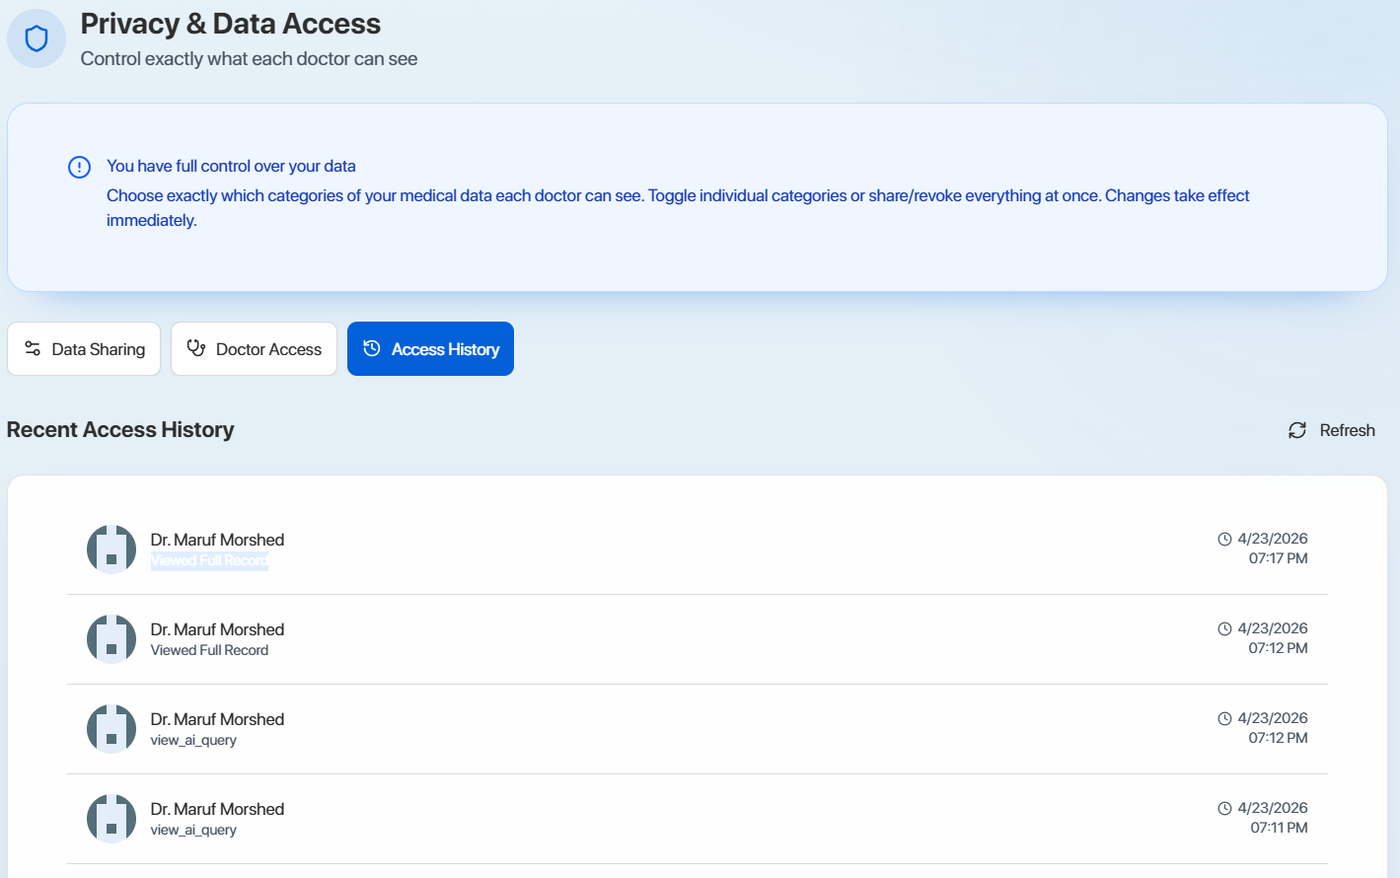
\includegraphics[height=6.0cm]{figures-ui/ui_consent_audit.png}\hfill
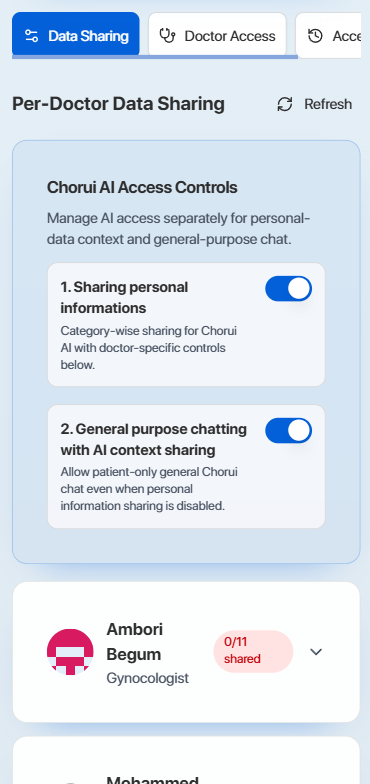
\includegraphics[height=6.0cm]{figures-ui/ui_mobile_consent.png}\\[3pt]
\figurepanellabel{\makebox[\textwidth]{(b) Patient-visible access log\hfill(c) Sharing controls at a phone viewport}}
\caption{The consent surface. Patients grant categories per recipient, revise them at any
time, and review clinician or assistant-mediated access in the audit log. Panel (c) shows
the same controls at a phone viewport.}
\label{fig:ui-consent}
\end{figure}

\begin{figure}[!htbp]
\centering
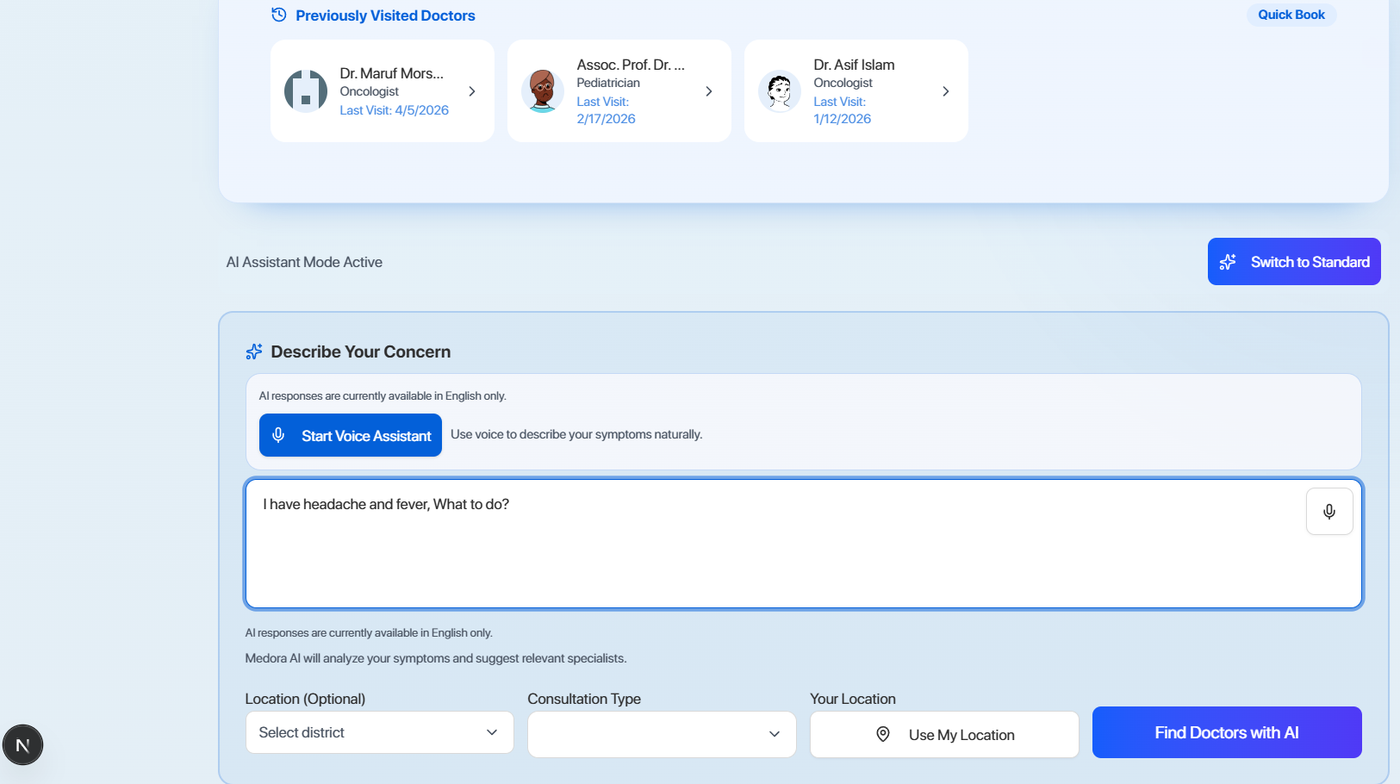
\includegraphics[width=0.80\textwidth]{figures-ui/ui_ai_navigation.png}\\[3pt]
\figurepanellabel{(a) Patient-facing specialty navigation}\vspace{6pt}
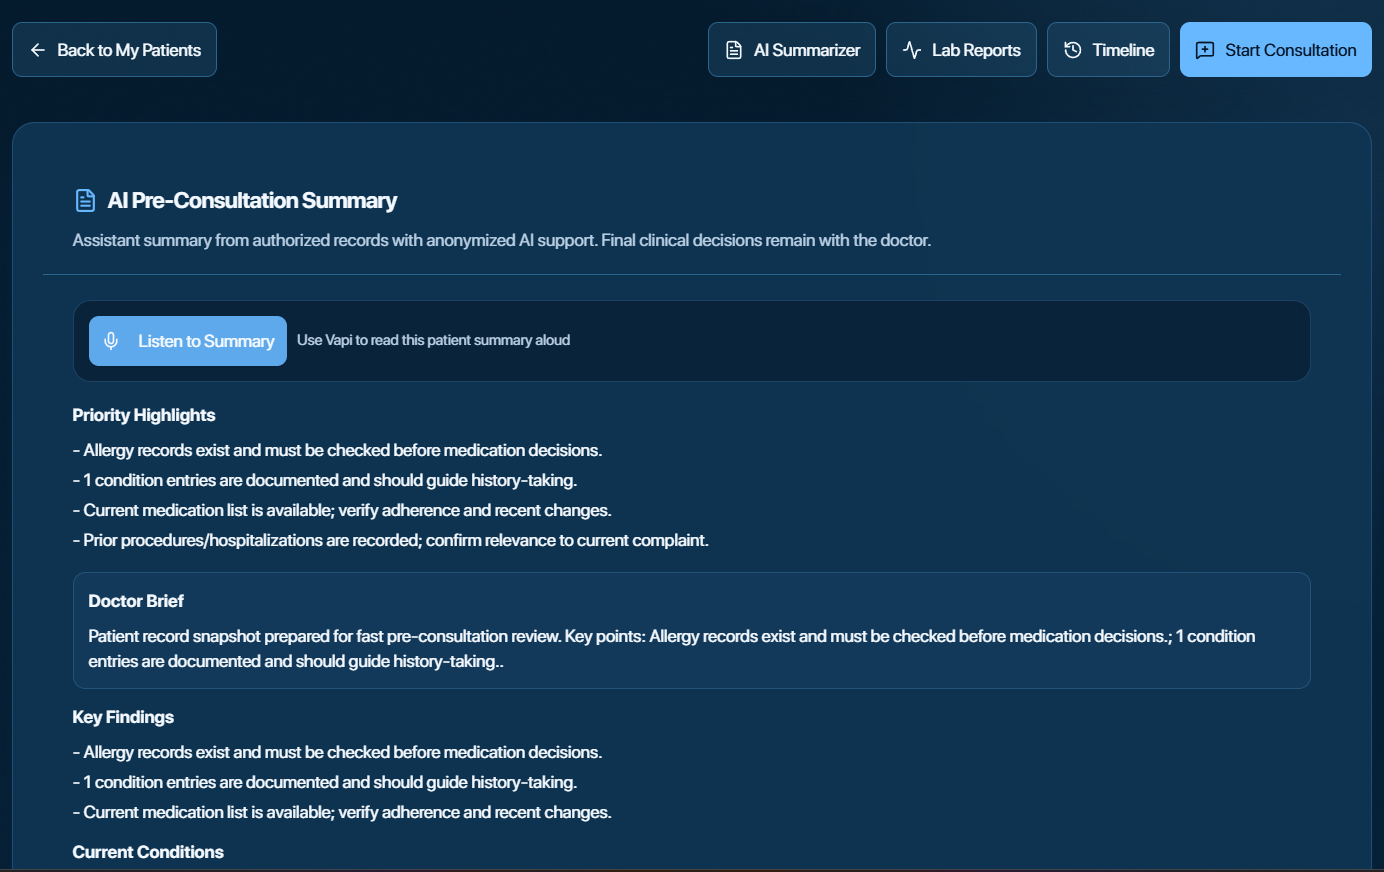
\includegraphics[height=6.0cm]{figures-ui/ui_ai_summary.png}\hfill
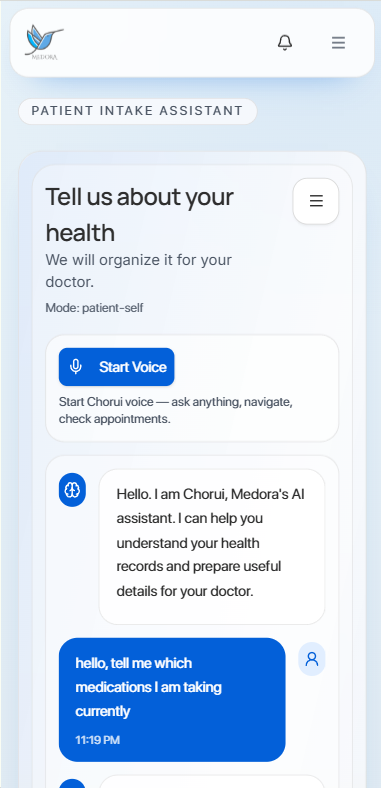
\includegraphics[height=6.0cm]{figures-ui/ui_mobile_assistant.png}\\[3pt]
\figurepanellabel{\makebox[\textwidth]{(b) Clinician-facing record summary\hfill(c) Assistant at a phone viewport}}
\caption{Assistive AI across patient and clinician roles. A typed or spoken condition can
launch specialty-oriented doctor discovery in (a); (b) organizes supplied records into a
source-linked clinician summary; and (c) provides mobile conversational access to Chorui.}
\label{fig:ui-ai}
\end{figure}

\textbf{Condition-to-doctor discovery.} Typed or spoken concerns produce specialty-oriented
candidates (Fig.~\ref{fig:ui-ai}a), with uncertainty and manual browsing retained.

\textbf{Registry-guided assistance.} A boundary fixture requests an administrator
dashboard; Chorui returns no destination because the registry excludes that route.

\textbf{Consent-scoped summarization.} A clinician receives an organized history containing
only shared categories (Fig.~\ref{fig:ui-consent}a). Withheld laboratory data are omitted
and marked unavailable; the patient can inspect the access log. Archived
\texttt{worked\_examples.json} illustrates these request contracts and boundaries,
rather than providing an additional accuracy benchmark.

\section{Impact}

Medora supports research into role-bounded navigation, consent granularity, bilingual
redaction and human review. The fixed registry and mock provider hold route access and
provider behaviour stable.

Patients manage records, discover doctors, book appointments and control sharing.
Clinicians review source-linked histories, intake, dictation and drafts. Chorui and Vapi
provide text/voice access through the installable PWA and reference deployment.

Reusable assets include the attributed medicine builder, region detection and OCR pipeline,
deterministic mock, registry, consent state machine, source attachment, and booking/outbox
patterns. Their documented contracts support reuse without adopting the full application.

Evidence covers software fixtures and one booking topology. Three endpoint groups have
task-level checks; six are documented capabilities. Further application-specific evaluation
can examine summary faithfulness, handwritten OCR, identifier and red-flag coverage,
and current medicine registration. Provider cost and retention depend on deployment.
Clinical trials, regulatory assessment and penetration testing remain outside this
software evaluation.

\section{Conclusions}

Medora integrates bilingual patient-held records, condition-driven doctor discovery,
transactional booking, and consent-gated text and voice assistance~\cite{medorasw}.
Its medicine builder, prescription prototype, and bounded workflows provide reusable
research components. Fixtures and attributed artifacts make evaluated behaviour inspectable,
while users review clinical drafts.

\section*{Ethics and data availability}
\label{sec:ethics}

Project-authored source retains its MIT notices; the optional combined detector
distribution uses AGPL-3.0 with corresponding source and preserved notices. Synthetic
fixtures and aggregate results use CC BY 4.0. The interface figures come from a non-production demonstration
deployment: the patient record belongs to a consenting author and the clinician entries are
test accounts.

The revision medicine build inventories five sources, using four for identity fields,
including Mendeley Data V1 under CC BY 4.0~\cite{bdmeds}. It excludes indication prose
and preserves row-level attribution and changes. The authors select multi-source public
distribution with documented reuse terms. A physician reviewed four sources and approximately
100 targeted entries on 29 September 2026: most mappings appeared reasonable; duplicates
and missing strengths were noted. This supports identity lookup, not prescribing,
whole-corpus accuracy, national completeness or current DGDA concordance.

The prescription image corpus is not deposited. Authors report public MedicalImage
Roboflow material and friend/family contributions consented for research, not image
redistribution. The authors report an author/institution decision permitting derived-weight release.
Verbal research consent was obtained; no formal institutional ethics review was obtained.
Images, private exports, and original notebook outputs remain excluded.
The model card distinguishes author-reported workspace version 2 from directly inspected
artifact metadata and records the remaining historical dataset-link limitations.

A licensed clinician reviewed all 30 navigation fixtures case by case, correcting two
Bengali red-flag presentations to emergency; the rules were extended to match. Every
decision is recorded.

\section*{CRediT authorship contribution statement}
\textbf{Sarwad Hasan Siddiqui:} Conceptualization,  Software, Data curation, Methodology, Validation, Visualization, Writing -- original draft. \textbf{Adiba Tahsin:} Software, Methodology, Data curation, Writing -- original draft. \textbf{Kazi Saeed Alam:} Conceptualization, Supervision, Resources, Validation, Writing -- review and editing. \textbf{Sk. Imran Hossain:} Supervision, Writing -- review and editing.

\section*{Declaration of Generative AI and AI-assisted technologies in the writing process}
During the preparation of this work, the authors used ChatGPT in order to improve the readability and language of the manuscript. After using this service, the authors reviewed and edited the content as needed and take full responsibility for the content of the published article.

\section*{Declaration of competing interest}
The clinician who reviewed the navigation fixtures is a sibling of the first author.
The authors declare no competing financial interests.

\section*{Funding}
This research received no specific grant from funding agencies in the public,
commercial, or not-for-profit sectors, and was self-funded.

\begin{thebibliography}{00}
\bibitem{openmrs} OpenMRS Community, Architecture, \url{https://devmanual.openmrs.org/technology/architecture/}, accessed 2026.
\bibitem{bahmni} Bahmni Coalition, Bahmni: Open Source EMR \& Hospital Information System, \url{https://www.bahmni.org/}, accessed 2026.
\bibitem{gnuhealth} GNU Solidario, GNU Health Hospital Information System documentation, \url{https://docs.gnuhealth.org/his/}, accessed 2026.
\bibitem{ahmed2014} T. Ahmed et al., eHealth and mHealth initiatives in Bangladesh: a scoping study, BMC Health Services Research 14 (2014) 260, \href{https://doi.org/10.1186/1472-6963-14-260}{doi:10.1186/1472-6963-14-260}.
\bibitem{khan2012} S.Z. Khan et al., Hopes and fears in implementation of electronic health records in Bangladesh, Electronic Journal of Information Systems in Developing Countries 54 (2012) 1--18, \href{https://doi.org/10.1002/j.1681-4835.2012.tb00387.x}{doi:10.1002/j.1681-4835.2012.tb00387.x}.
\bibitem{rxnorm} S. Liu, W. Ma, R. Moore, V. Ganesan, S. Nelson, RxNorm: prescription for electronic drug information exchange, IT Professional 7 (2005) 17--23, \href{https://doi.org/10.1109/MITP.2005.122}{doi:10.1109/MITP.2005.122}.
\bibitem{bdmeds} M.M. Rahman, M.M. Khan, Medicinal products in Bangladesh: a dataset of generic and brand names, dosage strengths, and manufacturers, Mendeley Data V1 (2024), \href{https://doi.org/10.17632/zhtvkny53n.1}{doi:10.17632/zhtvkny53n.1}.
\bibitem{whisper} A. Radford, J.W. Kim, T. Xu, G. Brockman, C. McLeavey, I. Sutskever, Robust speech recognition via large-scale weak supervision, in: Proc. ICML, 2023, pp. 28492--28518.
\bibitem{du2020} Y. Du et al., PP-OCR: A practical ultra lightweight OCR system, arXiv:2009.09941 (2020).
\bibitem{prescriptionocr} A. Datta et al., Preserving medical information from doctor's prescription ensuring relation among the terminology, Computers in Biology and Medicine 188 (2025) 109812, \href{https://doi.org/10.1016/j.compbiomed.2025.109812}{doi:10.1016/j.compbiomed.2025.109812}.
\bibitem{shing2021} H.-C. Shing et al., Towards clinical encounter summarization: Learning to compose discharge summaries from prior notes, arXiv:2104.13498 (2021).
\bibitem{tracsum} B. Chu, M. Li, S. Frihat, C. Gu, G. Lodde, E. Livingstone, N. Fuhr, TracSum: a new benchmark for aspect-based summarization with sentence-level traceability in medical domain, in: Proc. EMNLP, 2025, pp. 844--864, \href{https://doi.org/10.18653/v1/2025.emnlp-main.43}{doi:10.18653/v1/2025.emnlp-main.43}.
\bibitem{wallace2022} W. Wallace et al., The diagnostic and triage accuracy of digital and online symptom checker tools: a systematic review, npj Digital Medicine 5 (2022) 118, \href{https://doi.org/10.1038/s41746-022-00667-w}{doi:10.1038/s41746-022-00667-w}.
\bibitem{zhang2024clinicalsummary} R. Zhang et al., Adapted large language models can outperform medical experts in clinical text summarization, Nature Medicine 30 (2024), \href{https://doi.org/10.1038/s41591-024-02855-5}{doi:10.1038/s41591-024-02855-5}.
\bibitem{goh2025gpt4assistance} E. Goh et al., GPT-4 assistance for improvement of physician performance on patient care tasks: a randomized controlled trial, Nature Medicine (2025), \href{https://doi.org/10.1038/s41591-024-03456-y}{doi:10.1038/s41591-024-03456-y}.
\bibitem{khan2023banglahealthner} A.A. Khan et al., NERvous About My Health: Constructing a Bengali Medical Named Entity Recognition Dataset, Findings of EMNLP (2023) 5768--5774, \href{https://doi.org/10.18653/v1/2023.findings-emnlp.383}{doi:10.18653/v1/2023.findings-emnlp.383}.
\bibitem{campion2025diri} T.R. Campion et al., DIRI: Adversarial Patient Reidentification with Large Language Models for Evaluating Clinical Text Anonymization, AMIA Jt. Summits Transl. Sci. Proc. (2025) 355--364, \url{https://pmc.ncbi.nlm.nih.gov/articles/PMC12150728/}.
\bibitem{yang2025adversarial} Y. Yang, Q. Jin, F. Huang et al., Adversarial prompt and fine-tuning attacks threaten medical large language models, Nature Communications 16 (2025) 9011, \href{https://doi.org/10.1038/s41467-025-64062-1}{doi:10.1038/s41467-025-64062-1}.
\bibitem{fhirconsent} HL7 International, FHIR R5 Consent, \url{https://hl7.org/fhir/R5/consent.html}, accessed 2026.
\bibitem{ihepcf} IHE International, Privacy Consent on FHIR (PCF), \url{https://profiles.ihe.net/ITI/PCF/index.html}, accessed 2026.
\bibitem{gics2022} M. Bialke et al., A FHIR has been lit on gICS: facilitating the standardised exchange of informed consent in a large network of university medicine, BMC Medical Informatics and Decision Making 22 (2022) 335, \href{https://doi.org/10.1186/s12911-022-02081-4}{doi:10.1186/s12911-022-02081-4}.
\bibitem{ttp2024} M. Bialke, D. Stahl, T. Leddig, W. Hoffmann, The University Medicine Greifswald's Trusted Third Party Dispatcher: State-of-the-Art Perspective Into Comprehensive Architectures and Complex Research Workflows, JMIR Medical Informatics 12 (2024) e65784, \href{https://doi.org/10.2196/65784}{doi:10.2196/65784}.
\bibitem{consent2025} S. St\"aubert, A. Merzweiler, J. R\"omhild, S. Lang, M. Bialke, Consent Management 2.0: Empowering Patient Will in Medical Research and Care, Studies in Health Technology and Informatics 331 (2025) 133--141, \href{https://doi.org/10.3233/SHTI251389}{doi:10.3233/SHTI251389}.
\bibitem{gdpr} European Parliament and Council, Regulation (EU) 2016/679 (General Data Protection Regulation), \url{https://eur-lex.europa.eu/eli/reg/2016/679/oj}, accessed 2026.
\bibitem{mdr} European Parliament and Council, Regulation (EU) 2017/745 on medical devices, \url{https://eur-lex.europa.eu/eli/reg/2017/745/oj}, accessed 2026.
\bibitem{amg} Federal Ministry of Justice, German Medicinal Products Act (AMG), English translation, \url{https://www.gesetze-im-internet.de/englisch_amg/}, accessed 2026.
\bibitem{medorasw} S.H. Siddiqui, A. Tahsin, K.S. Alam, S.I. Hossain, Medora: A Consent-Aware Bilingual Platform for Healthcare Management and Consultation with Assistive AI, \ReleaseVersion{} [software], \ReleaseDOI.

\end{thebibliography}

\end{document}
